% \todo[inline]{minimal model abstracting caches, preemption and store buffer flushes independent from execution} \noindent

\section{Machine Model}

% intro

% Our abstract machine model of a x86 multiprocessor system is illustrated in Figure \ref{fig:machine:overview}.

%We will start by defining an abstract machine model of a multiprocessor system that allows stores to be reordered after loads.
%Since we are only concerned with the machine's behaviour as observed by assembly programs, the internal structure of any real processor's microarchitecture is a highly abstracted.
%To keep the state space of the resulting model checking problems as small as possible, we defined our model on the basis of a 16 bit, 1 register machine.

% consistent with amd/intel litmus tests

% as observed by assembly programs.

% to reduce the state space, while emulating the behaviour of a x86 multiprocessor system.

% * abstract machine model to investigate the interaction of parallel programs through shared memory.

We will start by defining a \CHANGE{minimal virtual} machine model of a multiprocessor system as observed by assembly programs.
% \CHANGE{
% abstracting caches (assuming cache-coherence) and interleaving the execution of
% }
To keep the state space of the resulting model checking problems as small as possible, it is based on a 16 bit architecture, using only a minimal set of registers and a radically reduced instruction set.

\begin{figure}[!h]
  \centering
  % layers
\pgfdeclarelayer{background}
\pgfdeclarelayer{foreground}
\pgfsetlayers{background, main, foreground}

% styles
\tikzstyle{box} = [draw, text centered, rounded corners]
\tikzstyle{register} = [box, fill=white, minimum height=2em, minimum width=4em]
\tikzstyle{processor} = [draw, fill=blue!10, rounded corners]
\tikzstyle{buffer} = [processor, fill=red!10]%, dashed]

% distances
\def\blockdist{3}
\def\borderdist{0.2}

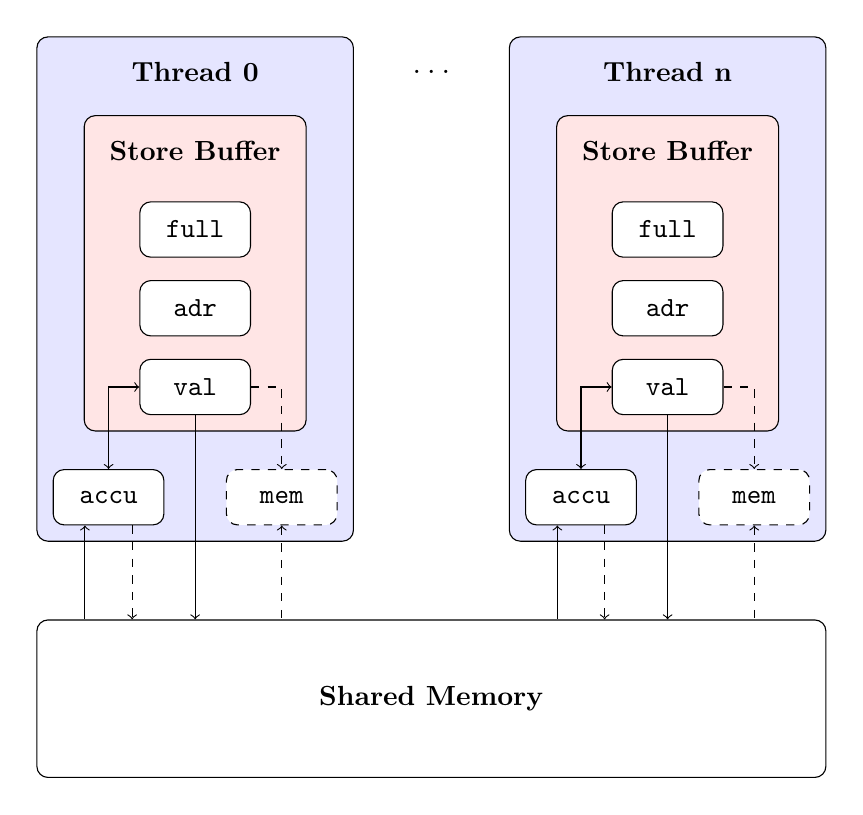
\begin{tikzpicture}

  % processor 0 %%%%%%%%%%%%%%%%%%%%%%%%%%%%%%%%%%%%%%%%%%%%%%%%%%%%%%%%%%%%%%%%
  \path (0, 0) node (title-0) [] {\textbf{Thread 0}};

  % store buffer
  \path (title-0)+(0, -1) node (sb-0) [] {\textbf{Store Buffer}};
  \path (sb-0)+(0, -1) node (full-0) [register] {\texttt{full}};
  \path (full-0)+(0, -1) node (adr-0) [register] {\texttt{adr}};
  \path (adr-0)+(0, -1) node (val-0) [register] {\texttt{val}};

  % registers
  \path (val-0)+(-1.1, -1.4) node (accu-0) [register] {\texttt{accu}};
  \path (val-0)+(1.1, -1.4) node (mem-0) [register, dashed] {\texttt{mem}};

  % paths
  \path [draw, <->] (val-0.west) -- (val-0.west -| accu-0.north) -- (accu-0.north);
  \path [draw, dashed, ->] (val-0.east) -- (val-0.east -| mem-0.north) -- (mem-0.north);

  \begin{pgfonlayer}{background}
    % bounding box
    \path (accu-0.west |- title-0.north)+(-\borderdist, \borderdist) node (a) {};
    \path (mem-0.south east)+(\borderdist, -\borderdist) node (b) {};
    \path [processor] (a) rectangle (b);

    % top left heap coordinate
    \path (a |- b)+(0, -1) node (tlh) {};

    % store buffer box
    \path (sb-0.north west)+(-\borderdist, \borderdist) node (a) {};
    \path (val-0.south -| sb-0.east)+(\borderdist, -\borderdist) node (b) {};
    \path [buffer] (a) rectangle (b);
  \end{pgfonlayer}

  % dots %%%%%%%%%%%%%%%%%%%%%%%%%%%%%%%%%%%%%%%%%%%%%%%%%%%%%%%%%%%%%%%%%%%%%%%
  \path (title-0)+(\blockdist, 0) node (dots) [] {\large $\ldots$};

  % processor n %%%%%%%%%%%%%%%%%%%%%%%%%%%%%%%%%%%%%%%%%%%%%%%%%%%%%%%%%%%%%%%%
  \path (dots)+(\blockdist, 0) node (title-n) [] {\textbf{Thread n}};

  % store buffer
  \path (title-n)+(0, -1) node (sb-n) [] {\textbf{Store Buffer}};
  \path (sb-n)+(0, -1) node (full-n) [register] {\texttt{full}};
  \path (full-n)+(0, -1) node (adr-n) [register] {\texttt{adr}};
  \path (adr-n)+(0, -1) node (val-n) [register] {\texttt{val}};

  % registers
  \path (val-n)+(-1.1, -1.4) node (accu-n) [register] {\texttt{accu}};
  \path (val-n)+(1.1, -1.4) node (mem-n) [register, dashed] {\texttt{mem}};

  % paths
  \path [draw, <->] (val-n.west) -- (val-n.west -| accu-n.north) -- (accu-n.north);
  \path [draw, dashed, ->] (val-n.east) -- (val-n.east -| mem-n.north) -- (mem-n.north);

  \begin{pgfonlayer}{background}
    % bounding box
    \path (accu-n.west |- title-n.north)+(-\borderdist, \borderdist) node (a) {};
    \path (mem-n.south east)+(\borderdist, -\borderdist) node (b) {};
    \path [processor] (a) rectangle (b);

    % bottom right heap coordinate
    \path (b)+(0, -\blockdist) node (brh) {};

    % store buffer box
    \path (sb-n.north west)+(-\borderdist, \borderdist) node (a) {};
    \path (val-n.south -| sb-n.east)+(\borderdist, -\borderdist) node (b) {};
    \path [buffer] (a) rectangle (b);
  \end{pgfonlayer}

  % heap %%%%%%%%%%%%%%%%%%%%%%%%%%%%%%%%%%%%%%%%%%%%%%%%%%%%%%%%%%%%%%%%%%%%%%%
  \path [box] (tlh) rectangle node (heap) [minimum height=2cm] {\textbf{Shared Memory}} (brh);

  % paths
  \path [draw, ->] (val-0) -- (heap.north -| val-0);
  \path [draw, <-, transform canvas={xshift=-3mm}] (accu-0) -- (heap.north -| accu-0);
  \path [draw, dashed, ->, transform canvas={xshift=3mm}] (accu-0) -- (heap.north -| accu-0);
  \path [draw, dashed, <-] (mem-0) -- (heap.north -| mem-0);

  \path [draw, ->] (val-n) -- (heap.north -| val-n);
  \path [draw, <-, transform canvas={xshift=-3mm}] (accu-n) -- (heap.north -| accu-n);
  \path [draw, dashed, ->, transform canvas={xshift=3mm}] (accu-n) -- (heap.north -| accu-n);
  \path [draw, dashed, <-] (mem-n) -- (heap.north -| mem-n);

\end{tikzpicture}

  \caption{Abstract Machine Model}
  \label{fig:machine:overview}
\end{figure}

A schematic overview is illustrated in Figure \ref{fig:machine:overview}, \CHANGE{where dashed lines depict components and data paths solely used by our \emph{compare and swap} mechanism}.
At the top of the figure are an arbitrary number of \CHANGE{logical} processors, each running a single \CHANGE{abstract} thread containing:

\begin{itemize}
  \item \ACCU: a single 16 bit accumulator register
  \item \MEM: a special purpose 16 bit register, storing the expected value required by a unary \emph{compare and swap} instruction
  % \item a \emph{store buffer} to break sequential consistency by delaying a single write, consisting of:
  \item a single element \emph{store buffer}, consisting of:
    \begin{itemize}
      \item \SBFULL: a one bit flag register, signaling that it contains a value and may be flushed
      \item \SBADR: a 16 bit address register
      \item \SBVAL: a 16 bit value register
    \end{itemize}
\end{itemize}

All \CHANGE{threads} are directly connected to the machine's shared memory, referred to as $\HEAP$, which will be uninitialized \CHANGE{unless any} eventual input data.
\CHANGE{Caches are abstracted as they don't influence
% our virtual machine's behaviour
the memory subsystem's basic behaviour
if they are coherent.}
In terms of memory ordering, the addition of a \emph{store buffer} allows stores to be reordered after loads, making our model consistent with Intel's or AMD's x86 memory ordering models \cite{ref:Intel, ref:AMD}.

% \bigskip
% \todo[inline]{model based on interleaving the execution of instructions and store buffer flushes}

\subsection*{Scheduling}

At each step \CHANGE{in time} a \CHANGE{single thread} either executes an instruction or flushes its store buffer back to memory.
Scheduling is generally performed non-deterministically under the following constraints.

\begin{enumerate}
  \item A \CHANGE{thread} can execute a read, modify or control operation at any time.
  \item A \CHANGE{thread} can voluntarily flush its store buffer to memory only if it is full.
  \item A \CHANGE{thread} can execute a write or barrier operation only if its store buffer is empty.
  % \item \CHANGE{A thread can only execute an instruction if it is not suspended} %(by a previous \lstASM{CHECK} statement).}
  % \item \CHANGE{A thread cannot execute any more instructions if it has been stopped.} % by a \lstASM{HALT}.}
\end{enumerate}

\CHANGE{
We argue that this interleaving semantic is sufficient for simulating the effects of real hardware, due to the execution of instructions and store buffer flushes being seen as independent.
A similar argument applies regarding preemption, assuming the presence of at least as many physical processors as running threads.
Since preemptive operating system kernels contain memory barriers when switching contexts, our thread centric view remains valid
% as the architectural state remains the same and the move to another physical processor just manifests as a store buffer flush.
% and the switch to another processor
and preemption
is just hidden behind a store buffer flush.
}

% \todo[inline]{checkpoints?}
% \todo[inline]{halted threads?}

\subsection*{Instructions}

Our machine uses a radically reduced instruction set that contains only the most substantial operations.
Instructions are stored separately for each thread and are therefore not contained in memory.
This abstraction allows the program counter to address instructions by their index, starting from zero.
To simplify the definition of operational semantics, instructions are labelled using the following attributes:

\begin{itemize}
  \item \textbf{modify} -- Modifies a register's content.
  \item \textbf{read} -- Reads from memory using \emph{store forwarding}: if $\SBFULL$ is set and $\SBADR$ equals the given target address, the value contained in $\SBVAL$ is read instead of the corresponding shared memory location.
  \item \textbf{write} -- Writes to the store buffer by setting $\SBFULL$ to true, $\SBADR$ to the given target address and $\SBVAL$ to the value contained in $\ACCU$.
  \item \textbf{barrier} -- Blocks execution if the store buffer is full ($\SBFULL$ is set). %memory barrier% - requires the store buffer to be flushed
  \item \textbf{atomic} -- Multiple operations performed as a single, \CHANGE{indivisible} instruction.% (implies barrier)
  \item \textbf{control} -- Modifies the order in which instructions are executed.
\end{itemize}

Due to the single register architecture, all instructions have at most one operand.
The following list shall give an overview of our machine's instruction set.

\newcommand{\defop}[3]{
  \paragraph{#1} \hfill #2
  \rule[0.5\baselineskip]{\textwidth}{0.1pt}\vspace{-0.5\baselineskip}\par\noindent
  #3
}

% \noindent
% \begin{tabu} to \textwidth {X[l]X[l]X[r]}
% \texttt{LOAD adr} & \texttt{accu = heap[adr]} & accu, read \\
% \texttt{STORE adr} & \texttt{heap[adr] = accu} & write
% \end{tabu}

\subsubsection*{Memory}

\CHANGE{
Two addressing modes are supported: direct and indirect denoted by square brackets (e.g. \lstASM{LOAD [arg]}).
}

\defop
{\lstASM{LOAD arg}}
{modify, read}
{Loads the value found at address \texttt{arg} into \ACCU.}

\defop
{\lstASM{STORE arg}}
{write}
{Stores the value found in $\ACCU$ at address \texttt{arg}.}

\defop
{\lstASM{FENCE}}
{barrier}
{Memory barrier.}

\subsubsection*{Arithmetic}

\CHANGE{
% \todo[inline]{say something about that all are unsigned and two's-compliment}
% Interpretation of a value's signedness is left to the programmmer.
% All values may be interpreted as unsigned or signed according to two's compliment.
Since the interpretation of a value's signedness is left to the programmer, we only included the most basic arithmetic instructions, which are equivalent for unsigned and two's compliment representations.
Division is therefore left out due to its different implementations for signed and unsigned integers.
% For example, division is left out on purpose, since it would require different
}

\defop
{\lstASM{ADD arg}}
{modify, read}
{Adds the value found at address \texttt{arg} to \ACCU.}

\defop
{\lstASM{ADDI arg}}
{modify}
{Adds the immediate value \texttt{arg} to \ACCU.}

\defop
{\lstASM{SUB arg}}
{modify, read}
{Subtracts the value found at address \texttt{arg} from \ACCU.}

\defop
{\lstASM{SUBI arg}}
{modify}
{Subtracts the immediate value \texttt{arg} from \ACCU.}

\defop
{\lstASM{MUL arg}}
{modify, read}
{Multiplies $\ACCU$ with the value found at address \texttt{arg}.}

\defop
{\lstASM{MULI arg}}
{modify}
{Multiplies $\ACCU$ with the immediate value \texttt{arg}.}

% ~\\\noindent
% \todo[inline]{\texttt{DIV} left because it's varying semantics in terms of signedness}
% Division instructions are omitted due to the varying semantics in terms of signedness.

\subsubsection*{Control Flow}

% \defop
% {\lstASM{CMP arg}}
% {modify, read}
% {Compares $\ACCU$ to the value found at address \texttt{arg} by performing an unsigned subtraction.}

\defop
{\lstASM{JMP arg}}
{control}
{Jumps to the statement at \texttt{arg} unconditionally.}

\defop
{\lstASM{JZ arg}}
{control}
{Jumps to the statement at \texttt{arg} if $\ACCU$ is zero.}

\defop
{\lstASM{JNZ arg}}
{control}
{Jumps to the statement at \texttt{arg} if $\ACCU$ is non-zero.}

\defop
{\lstASM{JS arg}}
{control}
{Jumps to the statement at \texttt{arg} if $\ACCU$ is negative according to two's compliment (most significant bit is set).}

\defop
{\lstASM{JNS arg}}
{control}
{Jumps to the statement at \texttt{arg} if $\ACCU$ is zero or positive according to two's compliment (most significant bit is unset).}

\defop
{\lstASM{JNZNS arg}}
{control}
{Jumps to the statement at \texttt{arg} if $\ACCU$ is positive according to two's compliment (non-zero and most significant bit is unset).}

\subsubsection*{Atomic}

% \todo[inline]{motivate}
% \noindent
\CHANGE{
We included a basic atomic \emph{compare and swap} operation, commonly used to implement synchronization primitives like semaphores and mutexes, as well as lockless data structures.
Since this particular command requires at least two operands (the target address and expected previous value), it had to be split up into two instructions due to our machine's unary input language.
% Due to the unary nature of our instruction format,
}

\defop
{\lstASM{MEM arg}}
{modify, mem, read}
{Loads the value \CHANGE{from} address \texttt{arg} into $\ACCU$ and $\MEM$ as the expectation during a latter \emph{compare and swap} operation.}

\defop
{\lstASM{CAS arg}}
{modify, read, atomic, barrier}
{Atomically compares the expected value in $\MEM$ to the actual value found at address \texttt{arg} and only writes the value found in $\ACCU$ back to address \texttt{adr} if they are equal.
Acts like a memory barrier.
% \todo{explain why non-blocking}}
}

\subsubsection*{Termination}

% \todo[inline]{motivate}
\CHANGE{
% Explicit termination of a single thread or the whole machine can be issued by the following commands.
Explicitly stopping a single thread or terminating the whole machine can be achieved by the following commands.
}

\defop
{\lstASM{HALT}}
{barrier, control}
{Stops the current thread.}

\defop
{\lstASM{EXIT arg}}
{control}
{Stops the machine with exit code \texttt{arg}.}

\subsubsection*{Meta}

\CHANGE{
The following high-level meta instruction, mimicking a reverse semaphore (and therefore not available on real hardware),
shall simplify the implementation of so called \emph{checker threads}
% by mimicking common synchronization primitives
used to programmatically validate machine states at runtime.
% validate machine states at runtime.
}

\defop
{\lstASM{CHECK arg}}
{control}
{Synchronize on checkpoint \texttt{arg} \CHANGE{(rendezvous)}.
Suspends execution until all threads, containing a call to checkpoint \texttt{arg}, reached the corresponding \lstASM{CHECK} statement.}

% \newpage

\subsection*{Programs}

Each thread is programmed using an assembly style language, defined by the following syntax.

\begin{figure}[!h]
\begin{grammar}
\small

<int> ::= an integer number

<label> ::= a sequence of printable characters without "#"

<string> ::= a sequence of whitespace and printable characters without "#" and "\\n"

<comment> ::= "#" <string>

<nullary> ::= "FENCE" | "HALT"

<unary> ::= "ADDI" | "SUBI" | "MULI" | "EXIT" | "CHECK"

<memory> ::= "LOAD" | "STORE" | "ADD" | "SUB" | "MUL" | "CMP" | "MEM" | "CAS"

<jump> ::= "JMP" | "JZ" | "JNZ" | "JS" | "JNS" | "JNZNS"

<instruction> ::= <nullary>
\alt <unary> <int>
\alt <memory> ( <int> | "["<int>"]" )
\alt <jump> ( <int> | <label> )

<statement> ::= <label>":" <instruction> | <instruction>

<line> ::= <statement> | <statement> <comment> | <comment>

<program> ::= <line> | <line> "\\n" <program>
\end{grammar}
\caption{Program Syntax}
\label{fig:syntax:program}
\end{figure}

% If the final statement in a given program is no control instruction, a final \texttt{HALT} is inserted implicitly.
If the final statement in a given program is not an \lstASM{EXIT} instruction or unconditional \lstASM{JMP}, \CHANGE{an additional} \lstASM{HALT} is inserted implicitly.
